
\textit{Results from this chapter are preliminary and have not been reviewed yet by the LIGO Scientific Collaboration.}
%\newline

        \section{Directed TwoSpect}
        \label{directed}

TwoSpect performed aptly in Chapter~\ref{chap5}'s Mock Data Challenge, which warrants using the program to analyze the best existing GW data.
At the time of writing, the best consistent stretch of data remains Science Run 6 (S6) taken from 2009 July 09 to 2010 October 20 by LIGO Hanford Observatory (LHO) and LIGO Livingston Observatory (LLO).
Advanced LIGO (aLIGO) commissioning is already surpassing the sensitivity of S6 for short periods of time, but the data duration is too short for an analysis competitive with existing results~\cite{AbbottScoX12007}, in particular the 2011 Radiometer~\cite{AbadieStoch2011} high frequency results and 2014 TwoSpect~\cite{GoetzTwoSpectResults2014} low frequency results.

            %TwoSpect improvements myself (to do).

            \subsection{Targeted, directed and all-sky search sensitivity}
            \label{tradeoffs}

             %   Targeted (known object) vs directed (region)vs all-sky (everything).

            \subsection{Enhancements enabled by directed searching}
            \label{directed_enhancements}

             %   Modifications for directed search.

        \section{Quantifying directedness: sensitivity studies in real data}
        \label{quant_directed}


            %Quantify how good the improvements are in directed TwoSpect. 

            Cite Feldman-Cousins confidence intervals paper~\cite{FeldmanCousins1998}.

            Cite Ethan's thesis~\cite{RomeroThesis} and our paper, maybe by using generation functions to make better TwoSpect statistics.

      %\section{Real S6 data: statistics}

        \subsection{Real S6 data: detection efficiency}

\begin{figure}
\begin{center}
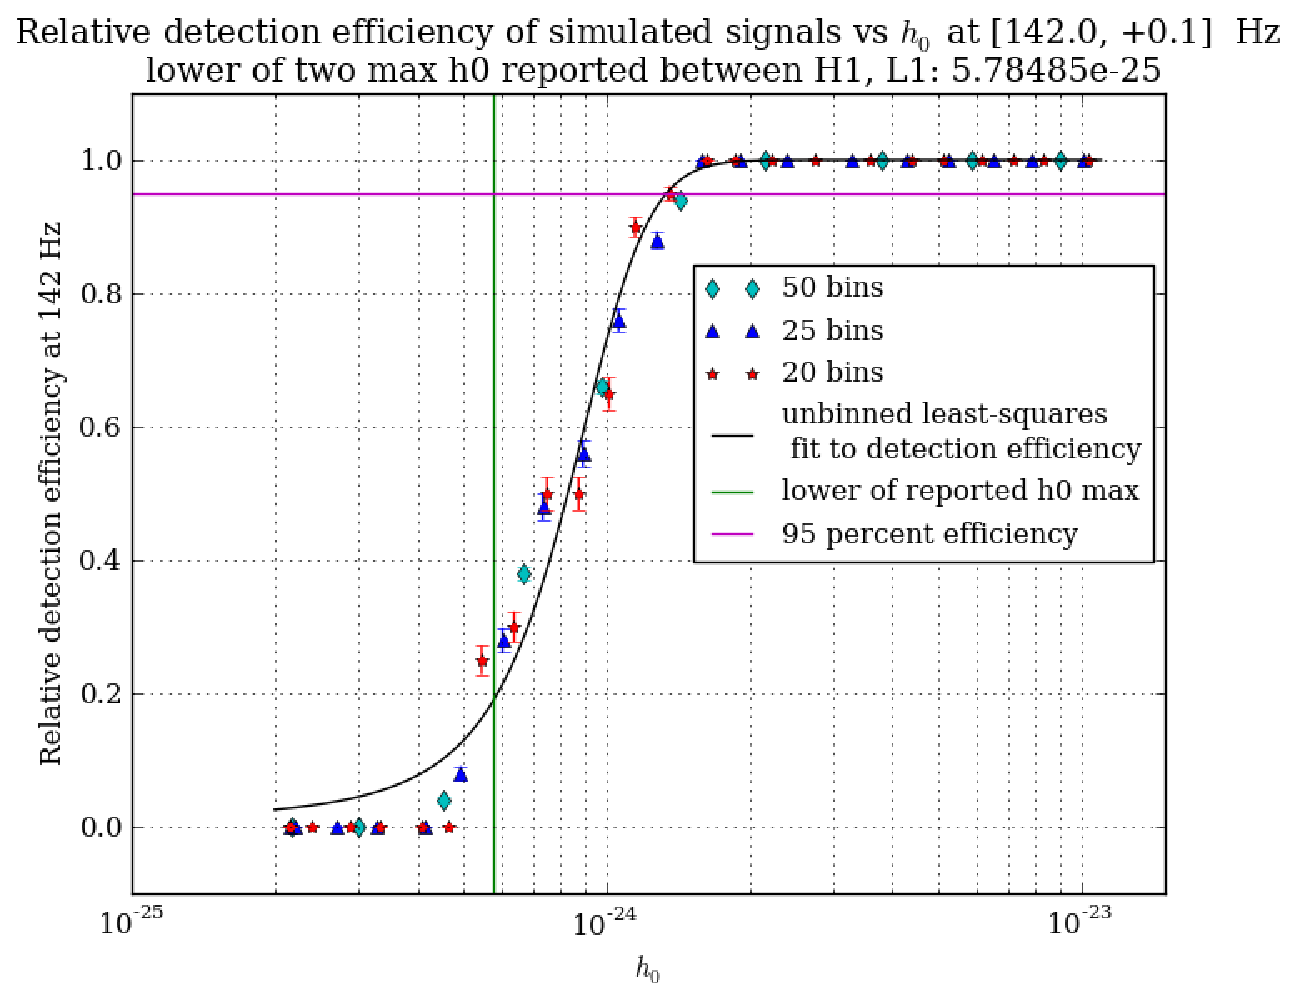
\includegraphics[width=0.4\paperwidth,height=0.2\paperheight]{plots/detectionEfficiencyh0-142-0Hz.eps}
\caption{Detection efficiency of 500 injections (each at H1, L1) into
S6 data at 142 Hz, given threshold log10p = -7.75}
\end{center}
\end{figure}

        \subsection{Real S6 data: $h_0$ recovered vs injected}

\begin{figure}
\begin{center}
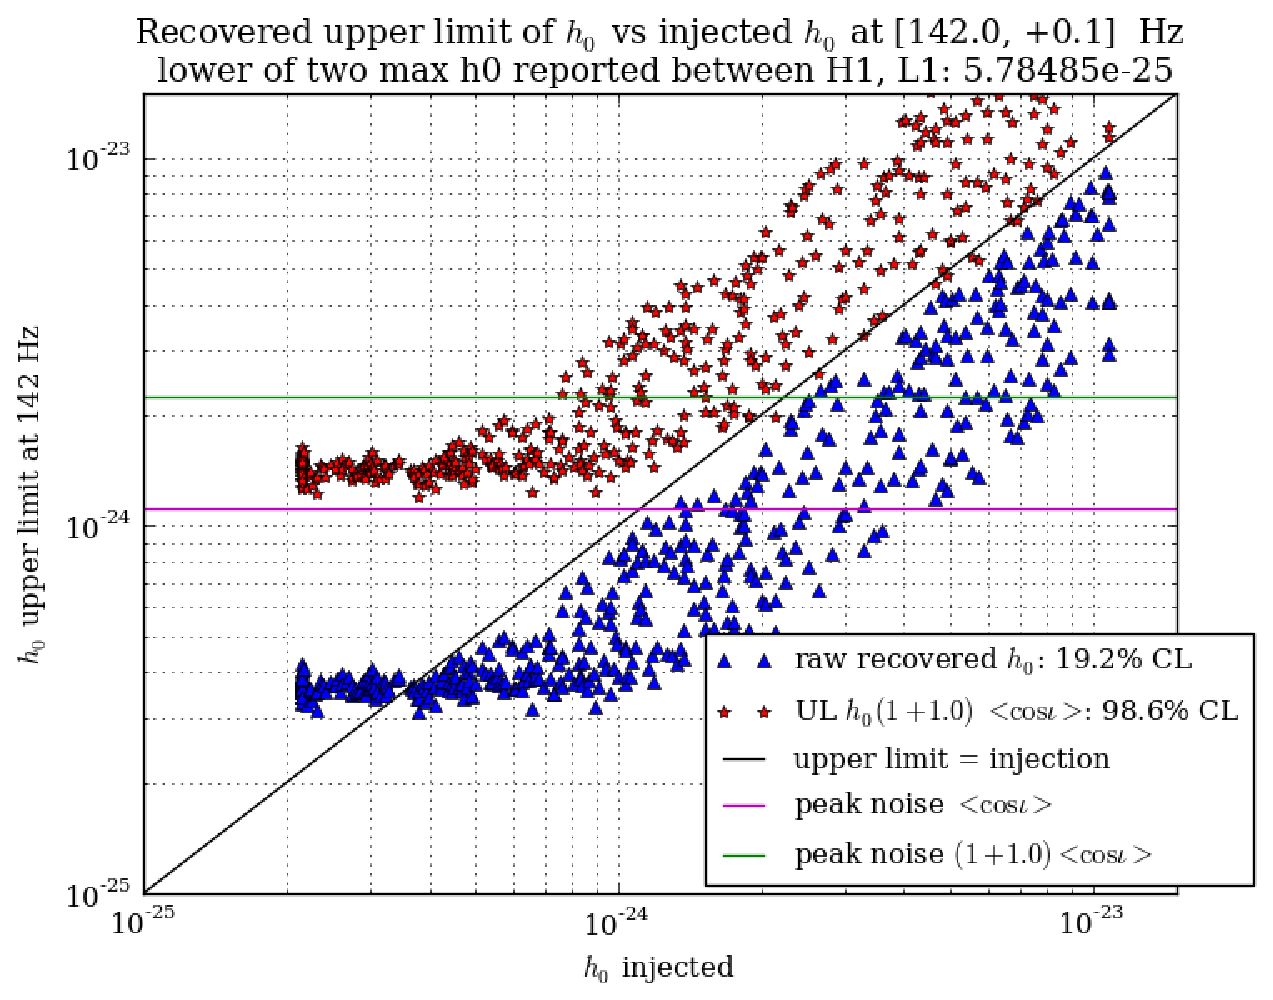
\includegraphics[width=0.4\paperwidth,height=0.2\paperheight]{plots/h0UL-vs-h0injected-142-0Hz.eps}
\caption{
Raw $h_0$ \& tentative 95\% confidence UL $>2\times10^{-24}$; 500 injections
into S6 data at 142 Hz (injections also done at 162, 222 Hz)}
\end{center}
\end{figure}

See Appendix~\ref{appendix2} for further injection studies.



%\section{S6: Scorpius X-1}

        \section{Scorpius X-1 search using Directed TwoSpect in S6}
        \label{directed_results}
 
            %Preliminary results of a directed search (possibly simulation-only).

            %We have a great deal of material here already, just need to pull from figures and commentary from the Sco X-1 wiki. Keith recommends paralleling the Sco X-1 paper.



\subsection{S6: Scorpius X-1 search plan}

\textbf{2 kHz, $\pm 3 \sigma_{a \sin i}$ search over all S6 data from H1 \& L1}
\begin{itemize}
\item Analyze 40 to 360 Hz with 840 s SFTs,
\item Analyze 360 to 2040 Hz with 360 s SFTs,\\
(to prevent spectral leakage)
\item Now planned: overlapping bands to verify
\item Search over 300+1100 Hz = 1.4 kHz complete on H1
\item Search over 300+1700 Hz = 2.0 kHz complete on L1
\end{itemize}


\subsection{S6: Scorpius X-1 heatmaps}

\begin{figure}
\begin{center}
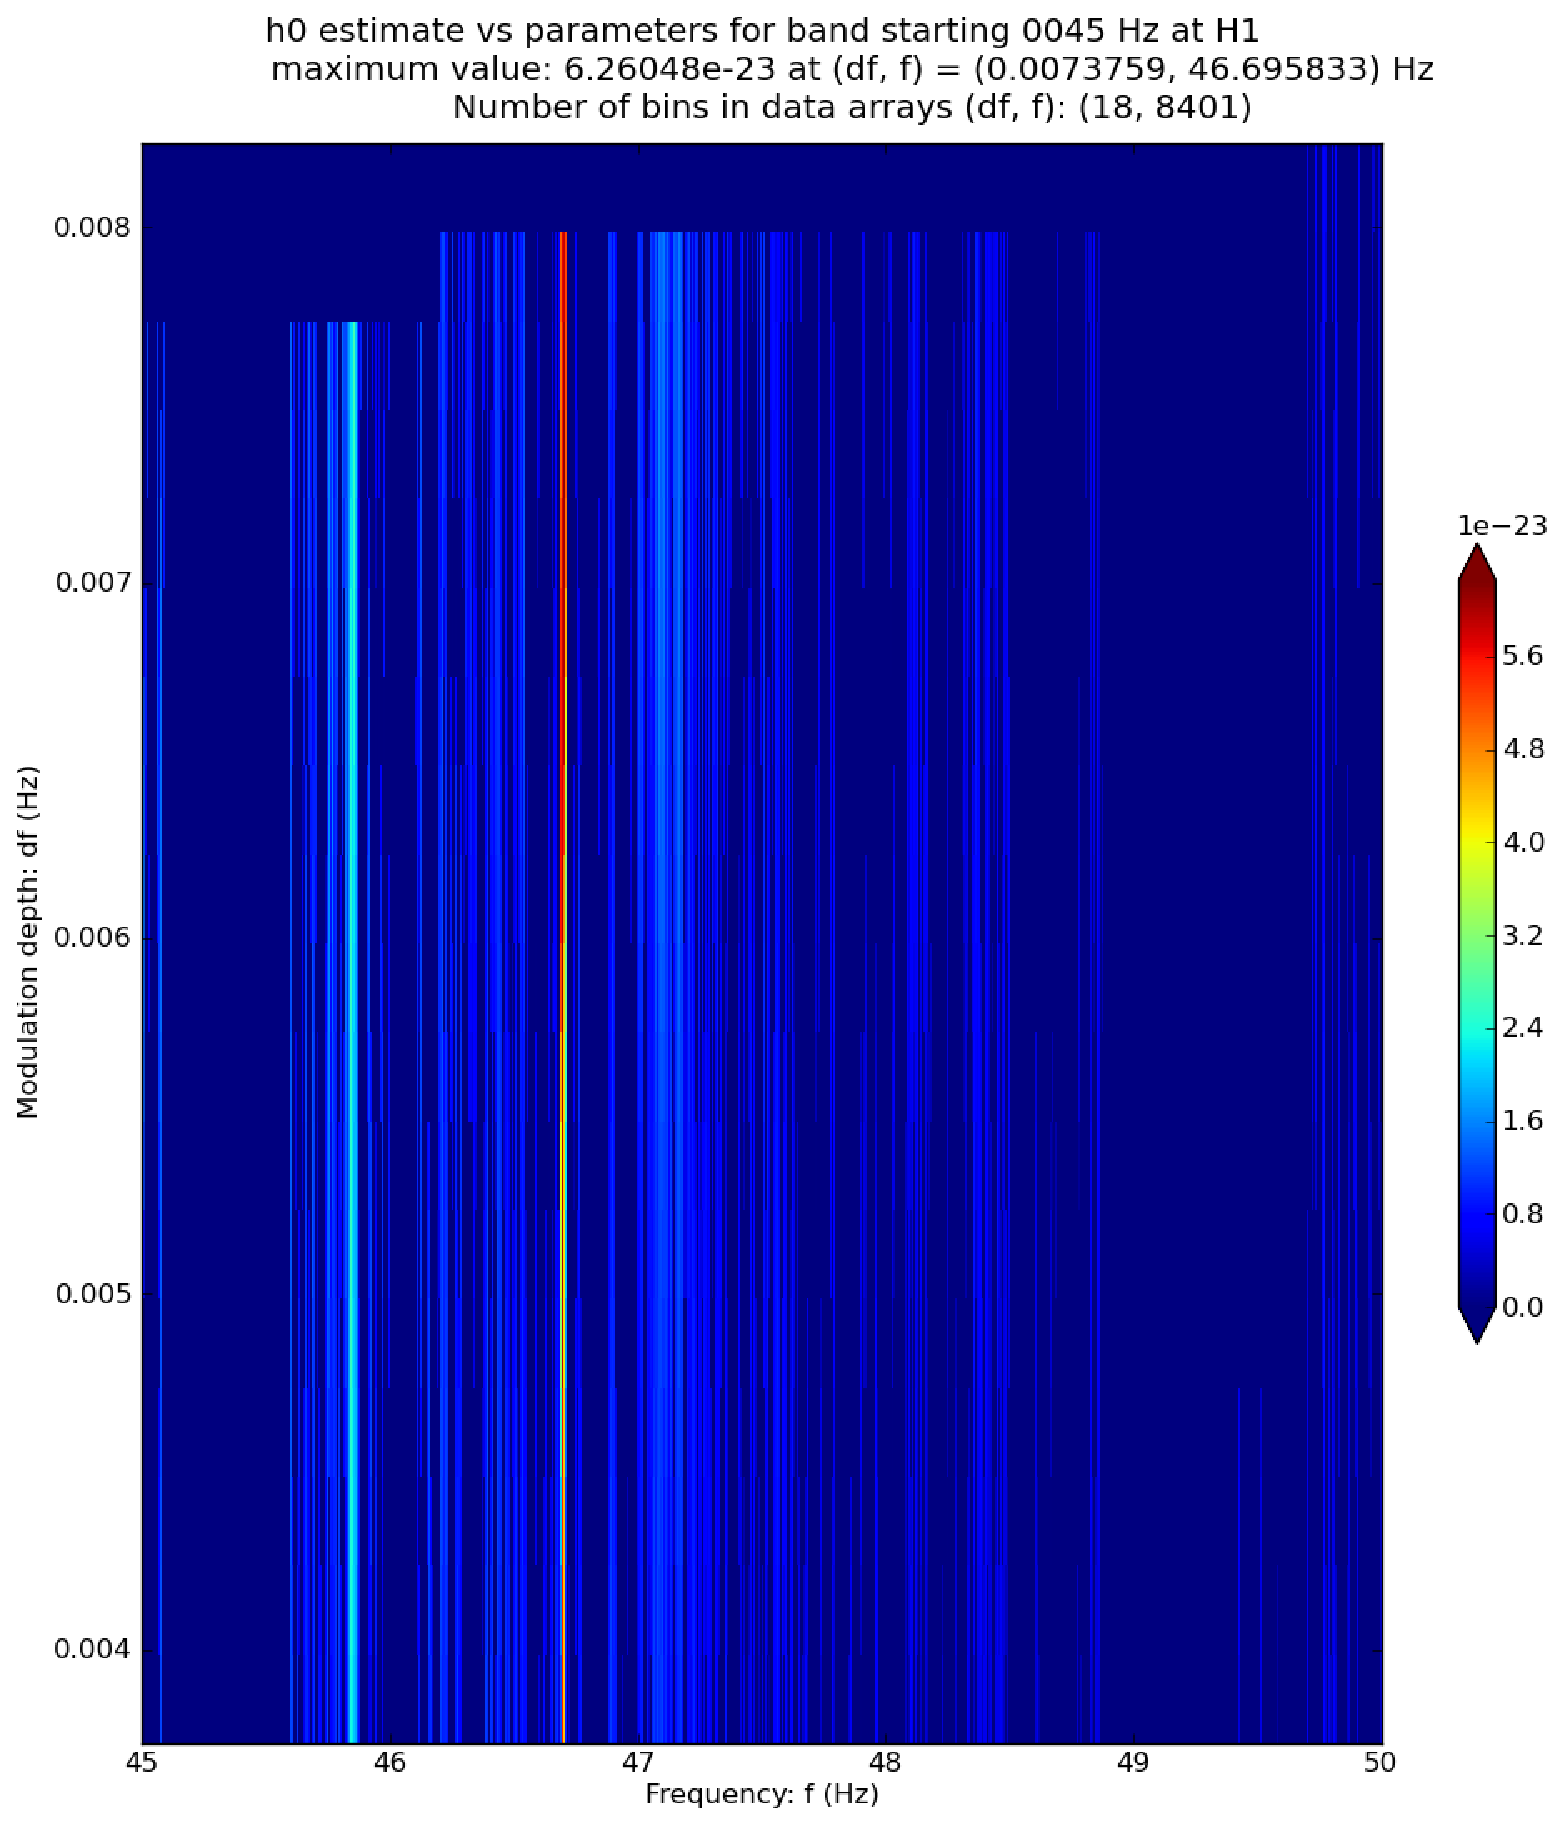
\includegraphics[width=0.4\paperwidth,height=0.2\paperheight]{plots/DFvsFresultsh0-H1_pulsar-0045.eps}
\caption{
S6 $h_0$ heatmap shows real data features, such as 46.7 Hz cal line}
\end{center}
\end{figure}

\subsection{S6: Scorpius X-1 upper limits, random polarization}

\begin{figure}
\begin{center}
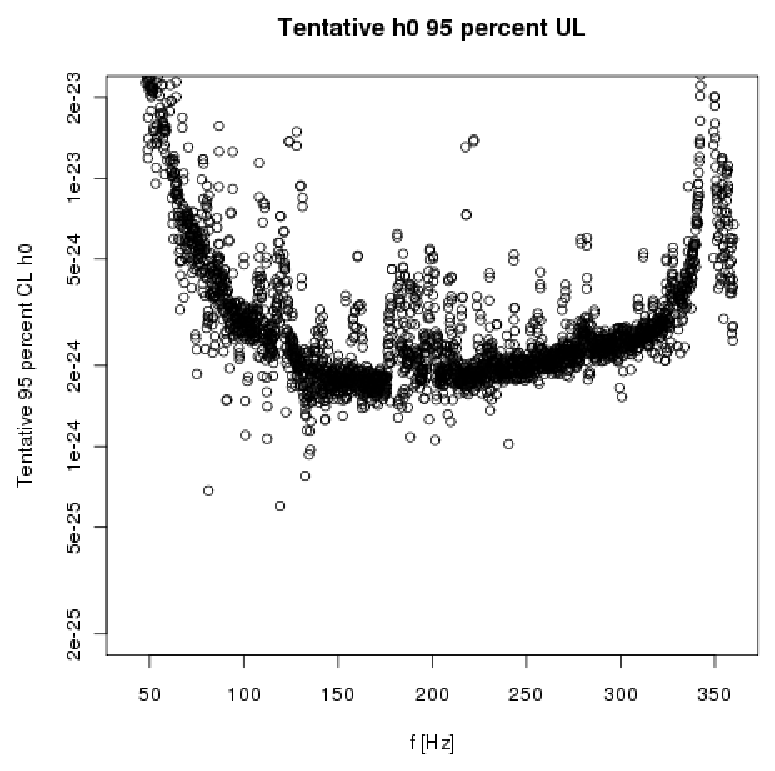
\includegraphics[width=0.4\paperwidth,height=0.2\paperheight]{plots/h0FullUL95logGuess-H1.eps}
\caption{
H1: loudest $h_0 \times \left( 1 + 0.8 \right) \times \left[\cos \iota \textup{ factor}\right]$ in 0.1 Hz bands}
\end{center}
\end{figure}

\begin{figure}
\begin{center}
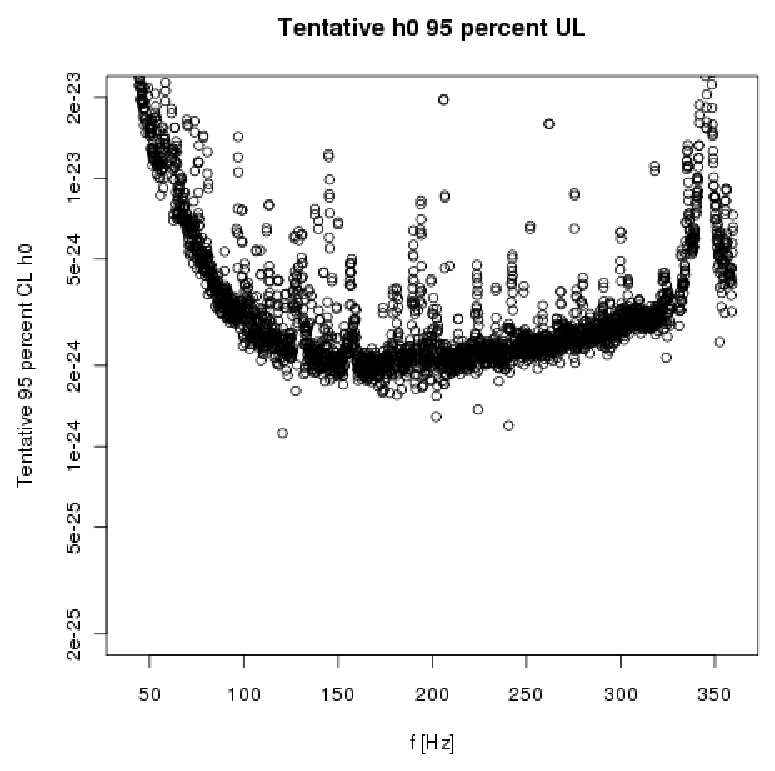
\includegraphics[width=0.4\paperwidth,height=0.2\paperheight]{plots/h0FullUL95logGuess-L1.eps}
\caption{
L1: loudest $h_0 \times \left( 1 + 0.8 \right) \times \left[\cos \iota \textup{ factor}\right]$ in 0.1 Hz bands}
\end{center}
\end{figure}

\begin{figure}
\begin{center}
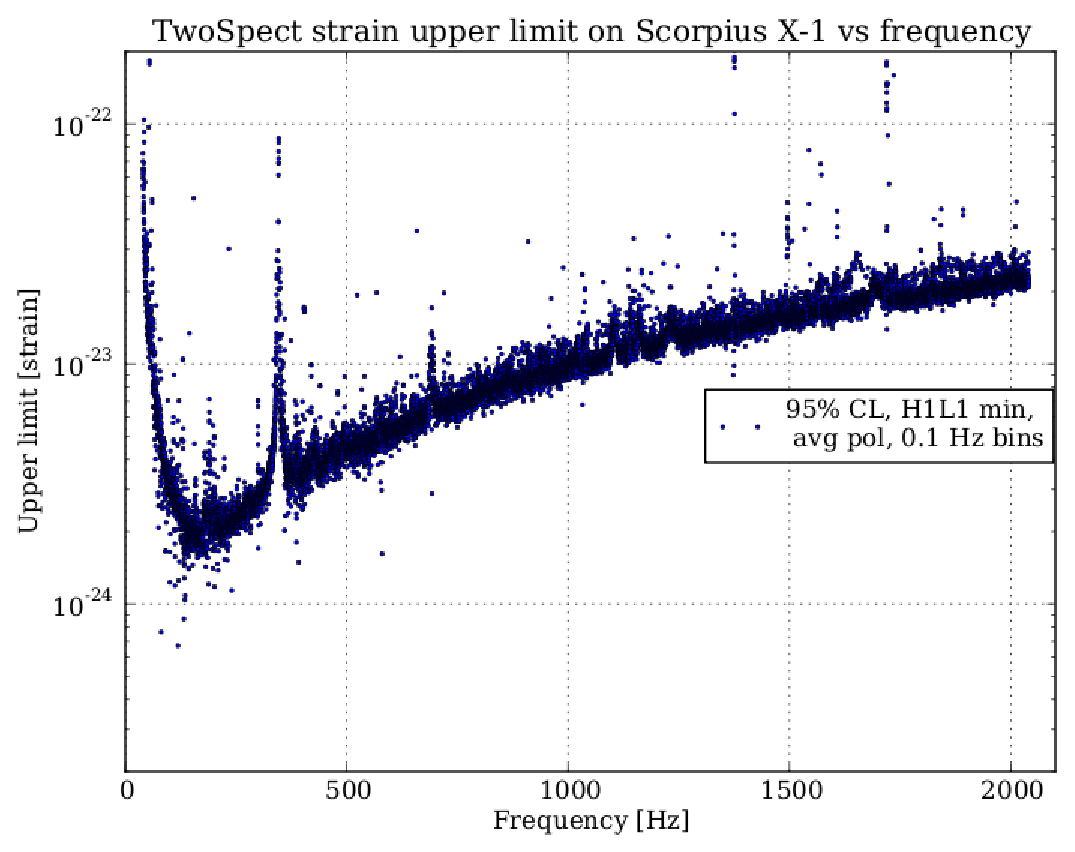
\includegraphics[width=0.8\paperwidth,height=0.4\paperheight]{plots/ScoX1ULs.eps}
\caption{
Joint upper limits for Scorpius X-1, using a confidence interval given by reported $h_0 \times \left( 1 + 1.0 \right) \times \left[\cos\iota \textup{ factor}\right]$ in 0.1 Hz bands. 
This spectrum covers 40 to 2040 Hz using the lower upper limit from either interferomer (H1 or L1) when both yielded data. 
A total of 28.8 Hz were in bands that yielded no real upper limit (because the quarter root of the test statistic was imaginary) in either interferometer, generally due to excessive noise in that band.
Bands were left-closed and right open, e.g., $\left[ 40.0,40.1\right), \left[ 40.1,40.2\right)\ldots \left[2039.9,2040.0\right)$.
}
\end{center}
\end{figure}

\subsection{S6: Scorpius X-1 outliers}

\begin{table}
\begin{center}
\begin{tabular}{r r l}
Outlier Number & Frequency (Hz) & Explanation \\
\hline
1 & 42.00 & \\
2 & 64.00 & \\
3 & 108.10 & \\
4 & 108.85 & \\
5 & 109.50 & \\
6 & 111.02 & \\
7 & 128.00 & \\
8 & 139.52 & \\
9 & 154.04 & \\
10 & 156.82 & \\
11 & 157.99 & \\
12 & 158.36 & \\
13 & 158.87 & \\
14 & 190.86 & \\
15 & 192.54 & Injected pulsar 8? \\
16 & 200.53 & \\
17 & 200.60 & \\
18 & 209.21 & \\
19 & 209.28 & \\
20 & 223.66 & \\
21 & 256.02 & \\
22 & 268.13 & \\
\end{tabular}
\caption{List of Scorpius X-1 outliers in the search of S6 data. This list covers 40 to 360 Hz.}
\label{ScoX1S6outlierTable}
\end{center}
\end{table}

Table~\ref{ScoX1S6outlierTable} presents a list of outliers present in both intereferometers.

\section{XTE J1751-305 search using Directed TwoSpect in S6}

\subsection{S6: XTE J1751-305 background}

Discovered by Markwardt et al in 2002~\cite{Markwardt2002}.

\textbf{XTE with shortest period, 42 minutes}\\
(P $\approx$$ $ 2545.3 s, $a \sin i$ $\approx0.010\pm0.003$s):\\
Search very fast ($< 10^5$ templates), promising target\\
\emph{although} estimated $d > 7$ kpc near galactic center
\\
$\textup{}$

\textbf{$\nu_0$}: 435.31799 Hz\\
\textbf{$r$-mode}: (2-0.5727597)*(435.31799 Hz) = 621.3034 Hz\\
$\textup{}$

\begin{description}
\item[{Searched frequencies}] [434.5,436.5] \& [620.5,622.5] Hz
\item{{Searching}} [869.5, 871.5]
\end{description}
$\rightarrow$ TwoSpect analysis, heatmaps done on $\nu_0$, $r$-mode\\
$\rightarrow$ Upper limits will be made

%\section{S6: XTE J1751-305}
\subsection{S6: XTE J1751-305 heatmaps}

\begin{figure}
\begin{center}
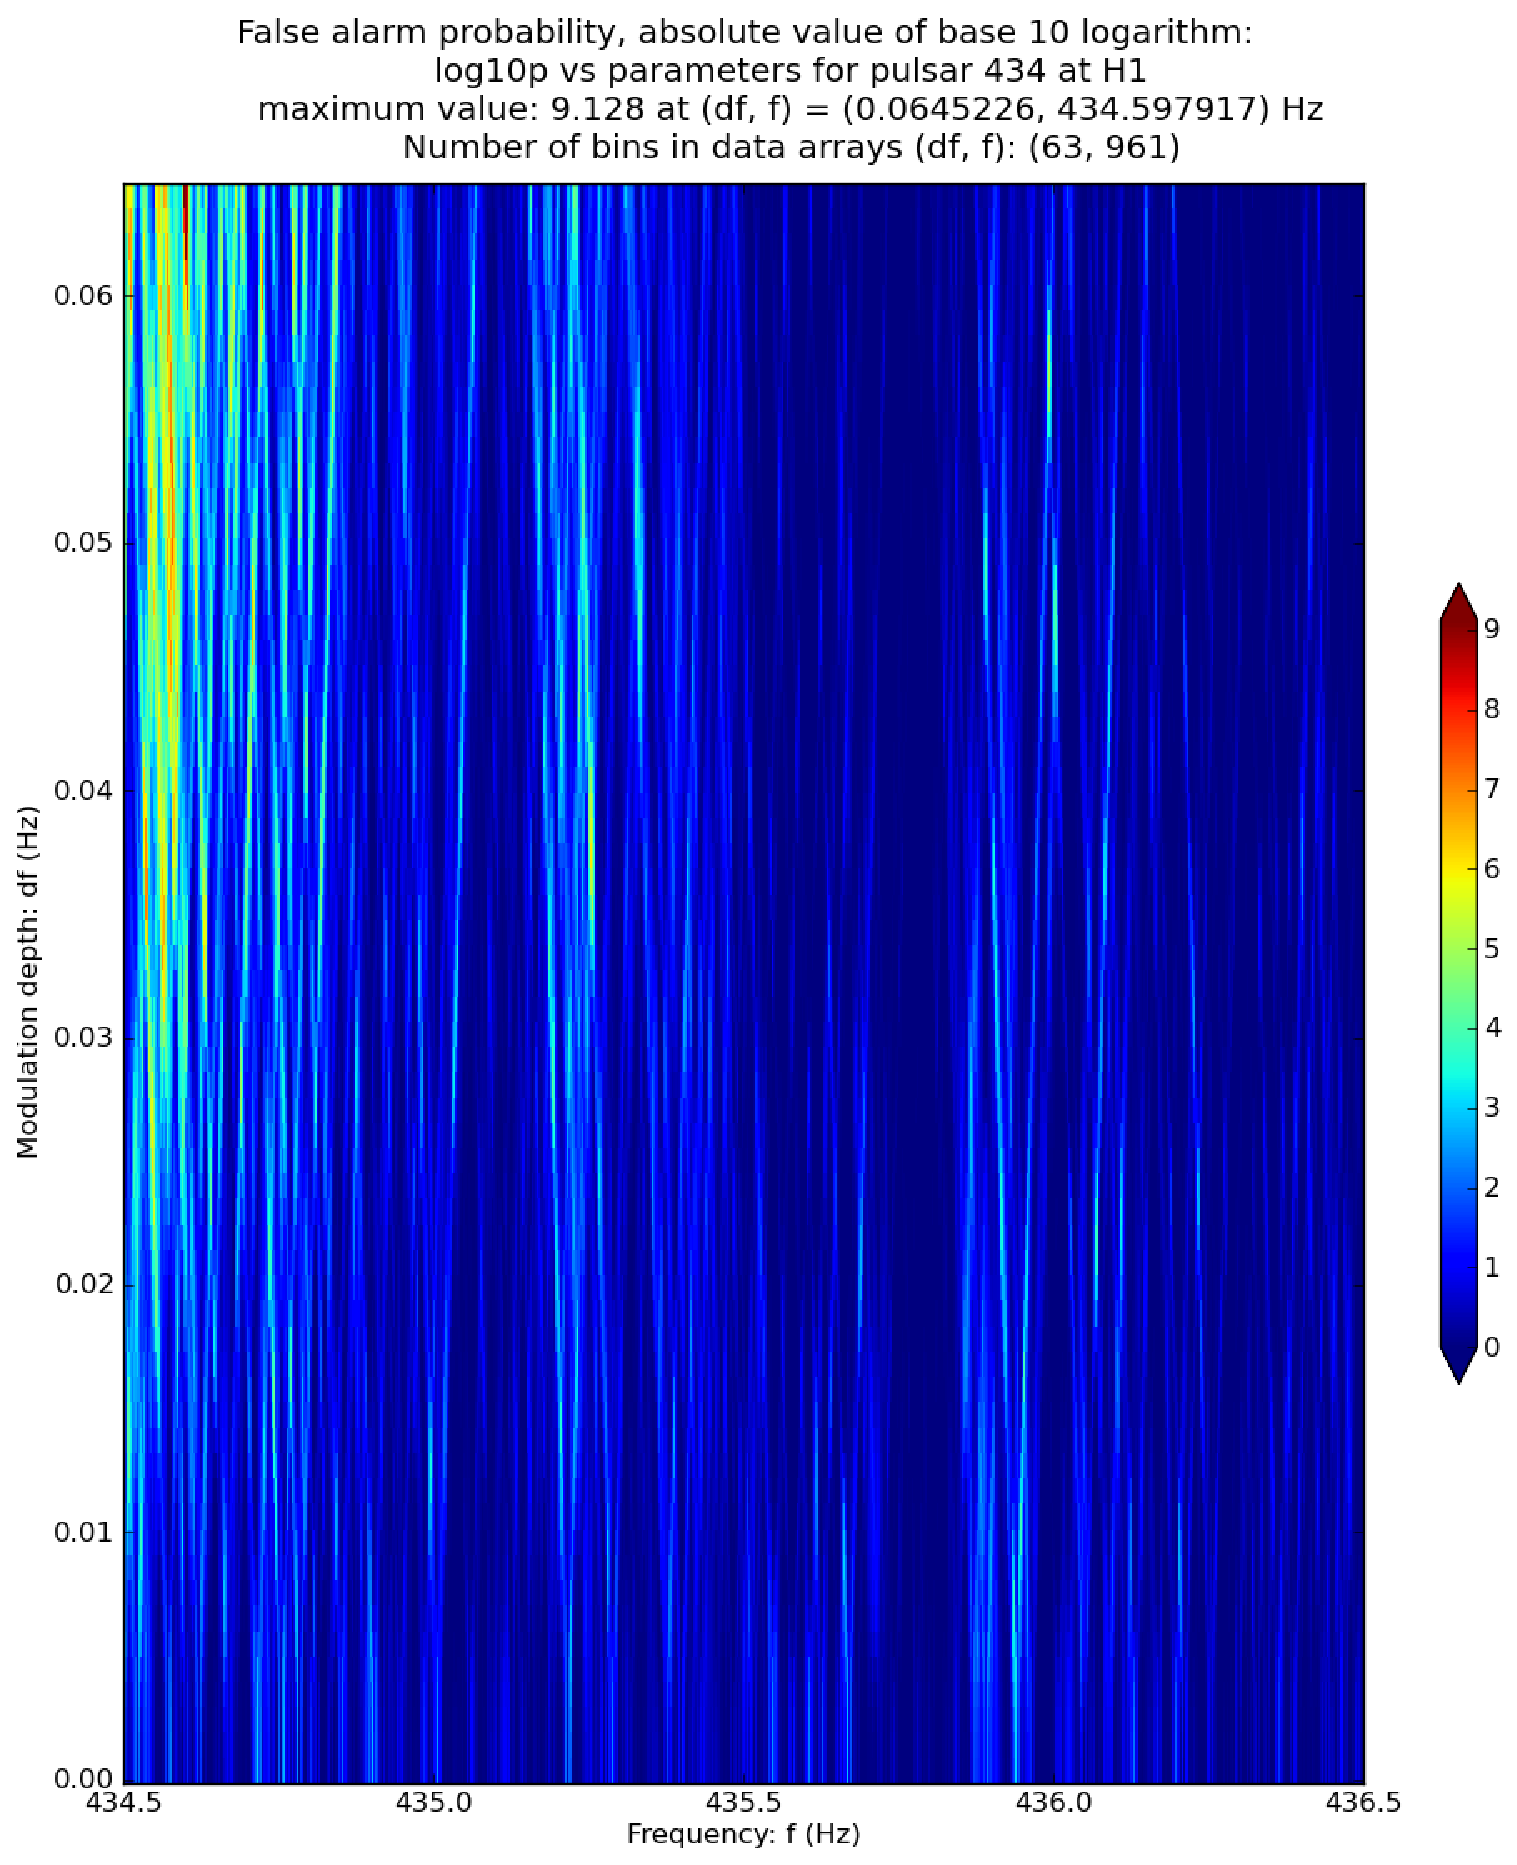
\includegraphics[width=0.4\paperwidth,height=0.2\paperheight]{plots/DFvsFresultsProb-H1_pulsar-434.eps}
\caption{
Quick look at J1751-305, H1 log10p, 435 Hz $\nu_0$}
\end{center}
\end{figure}


\begin{figure}
\begin{center}
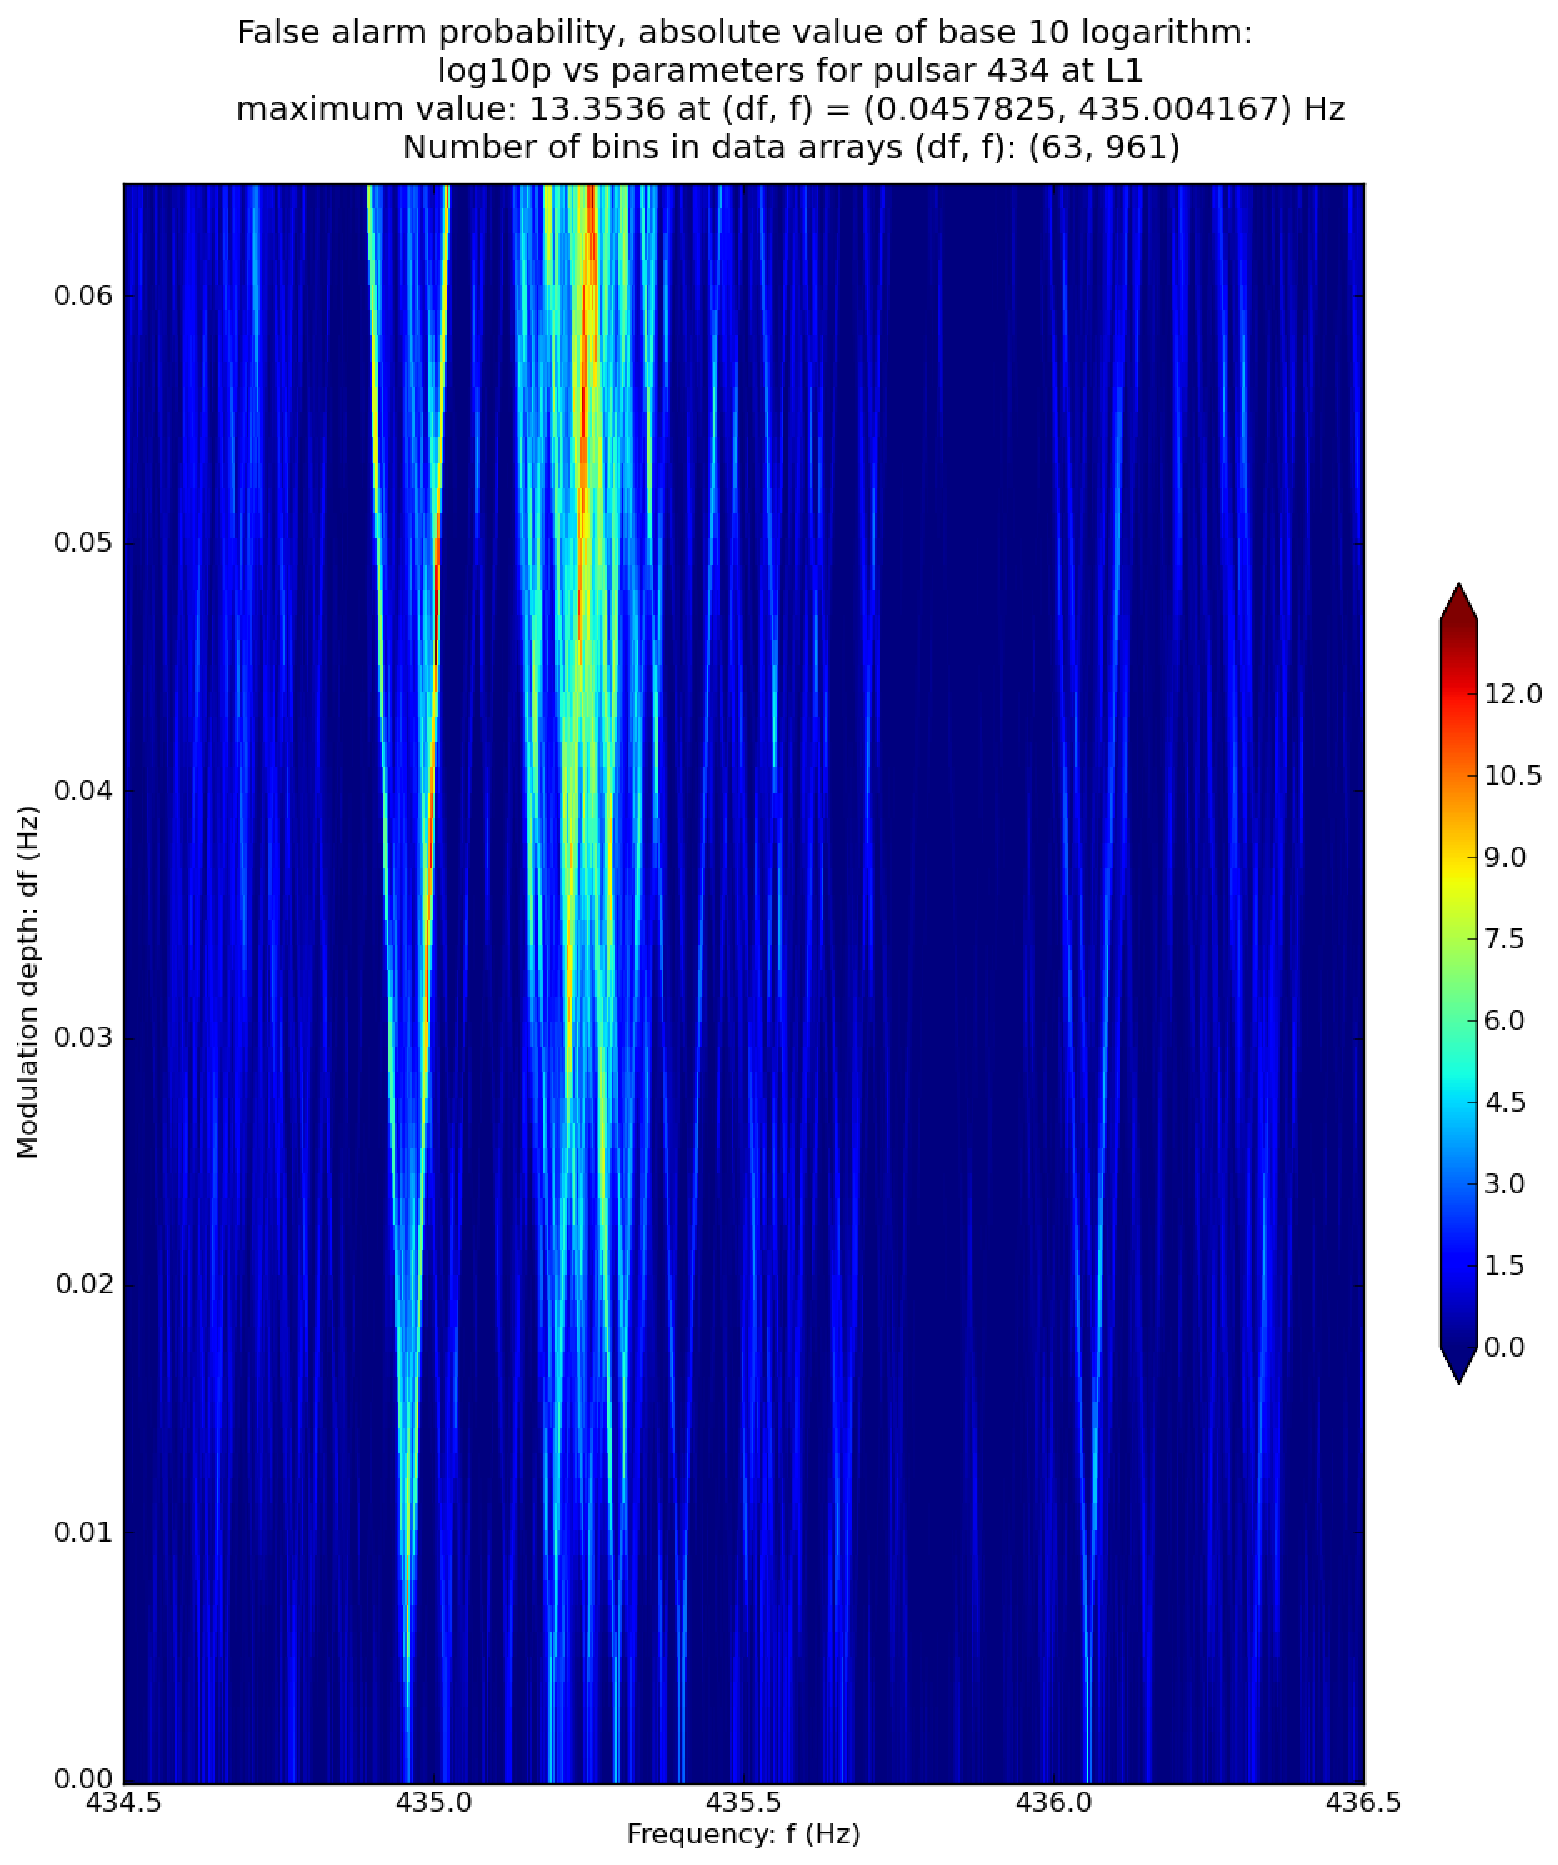
\includegraphics[width=0.4\paperwidth,height=0.2\paperheight]{plots/DFvsFresultsProb-L1_pulsar-434.eps}
\caption{
Quick look at J1751-305, L1 log10p, 435 Hz $\nu_0$}
\end{center}
\end{figure}


\begin{figure}
\begin{center}
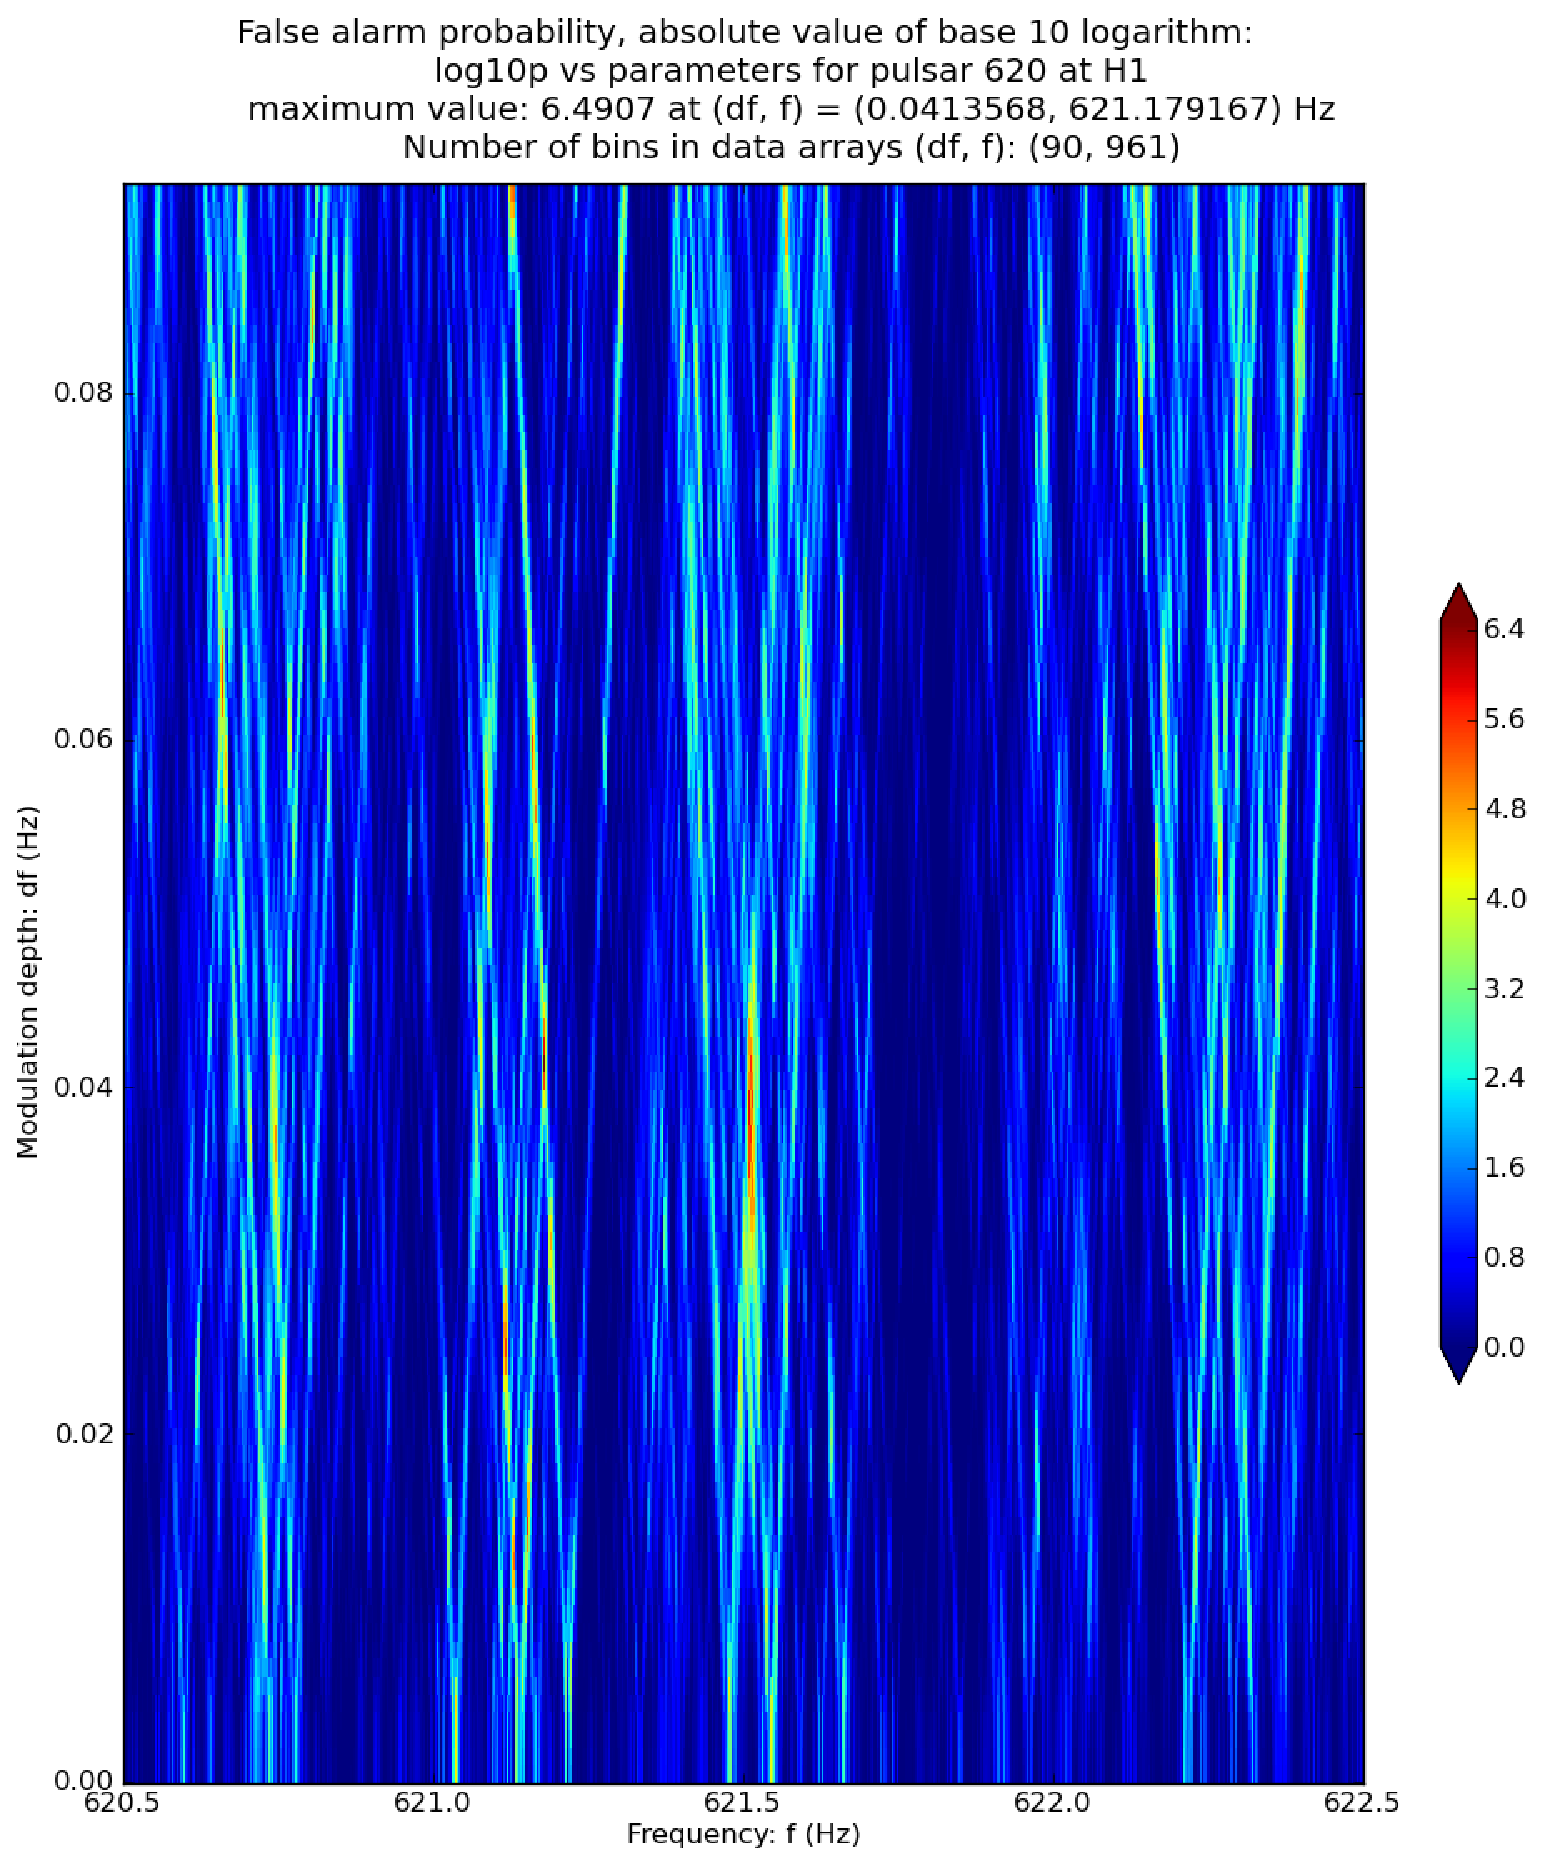
\includegraphics[width=0.4\paperwidth,height=0.2\paperheight]{plots/DFvsFresultsProb-H1_pulsar-620.eps}
\caption{
Quick look at J1751-305, H1 log10p, 621 Hz $r$-mode}
\end{center}
\end{figure}


\begin{figure}
\begin{center}
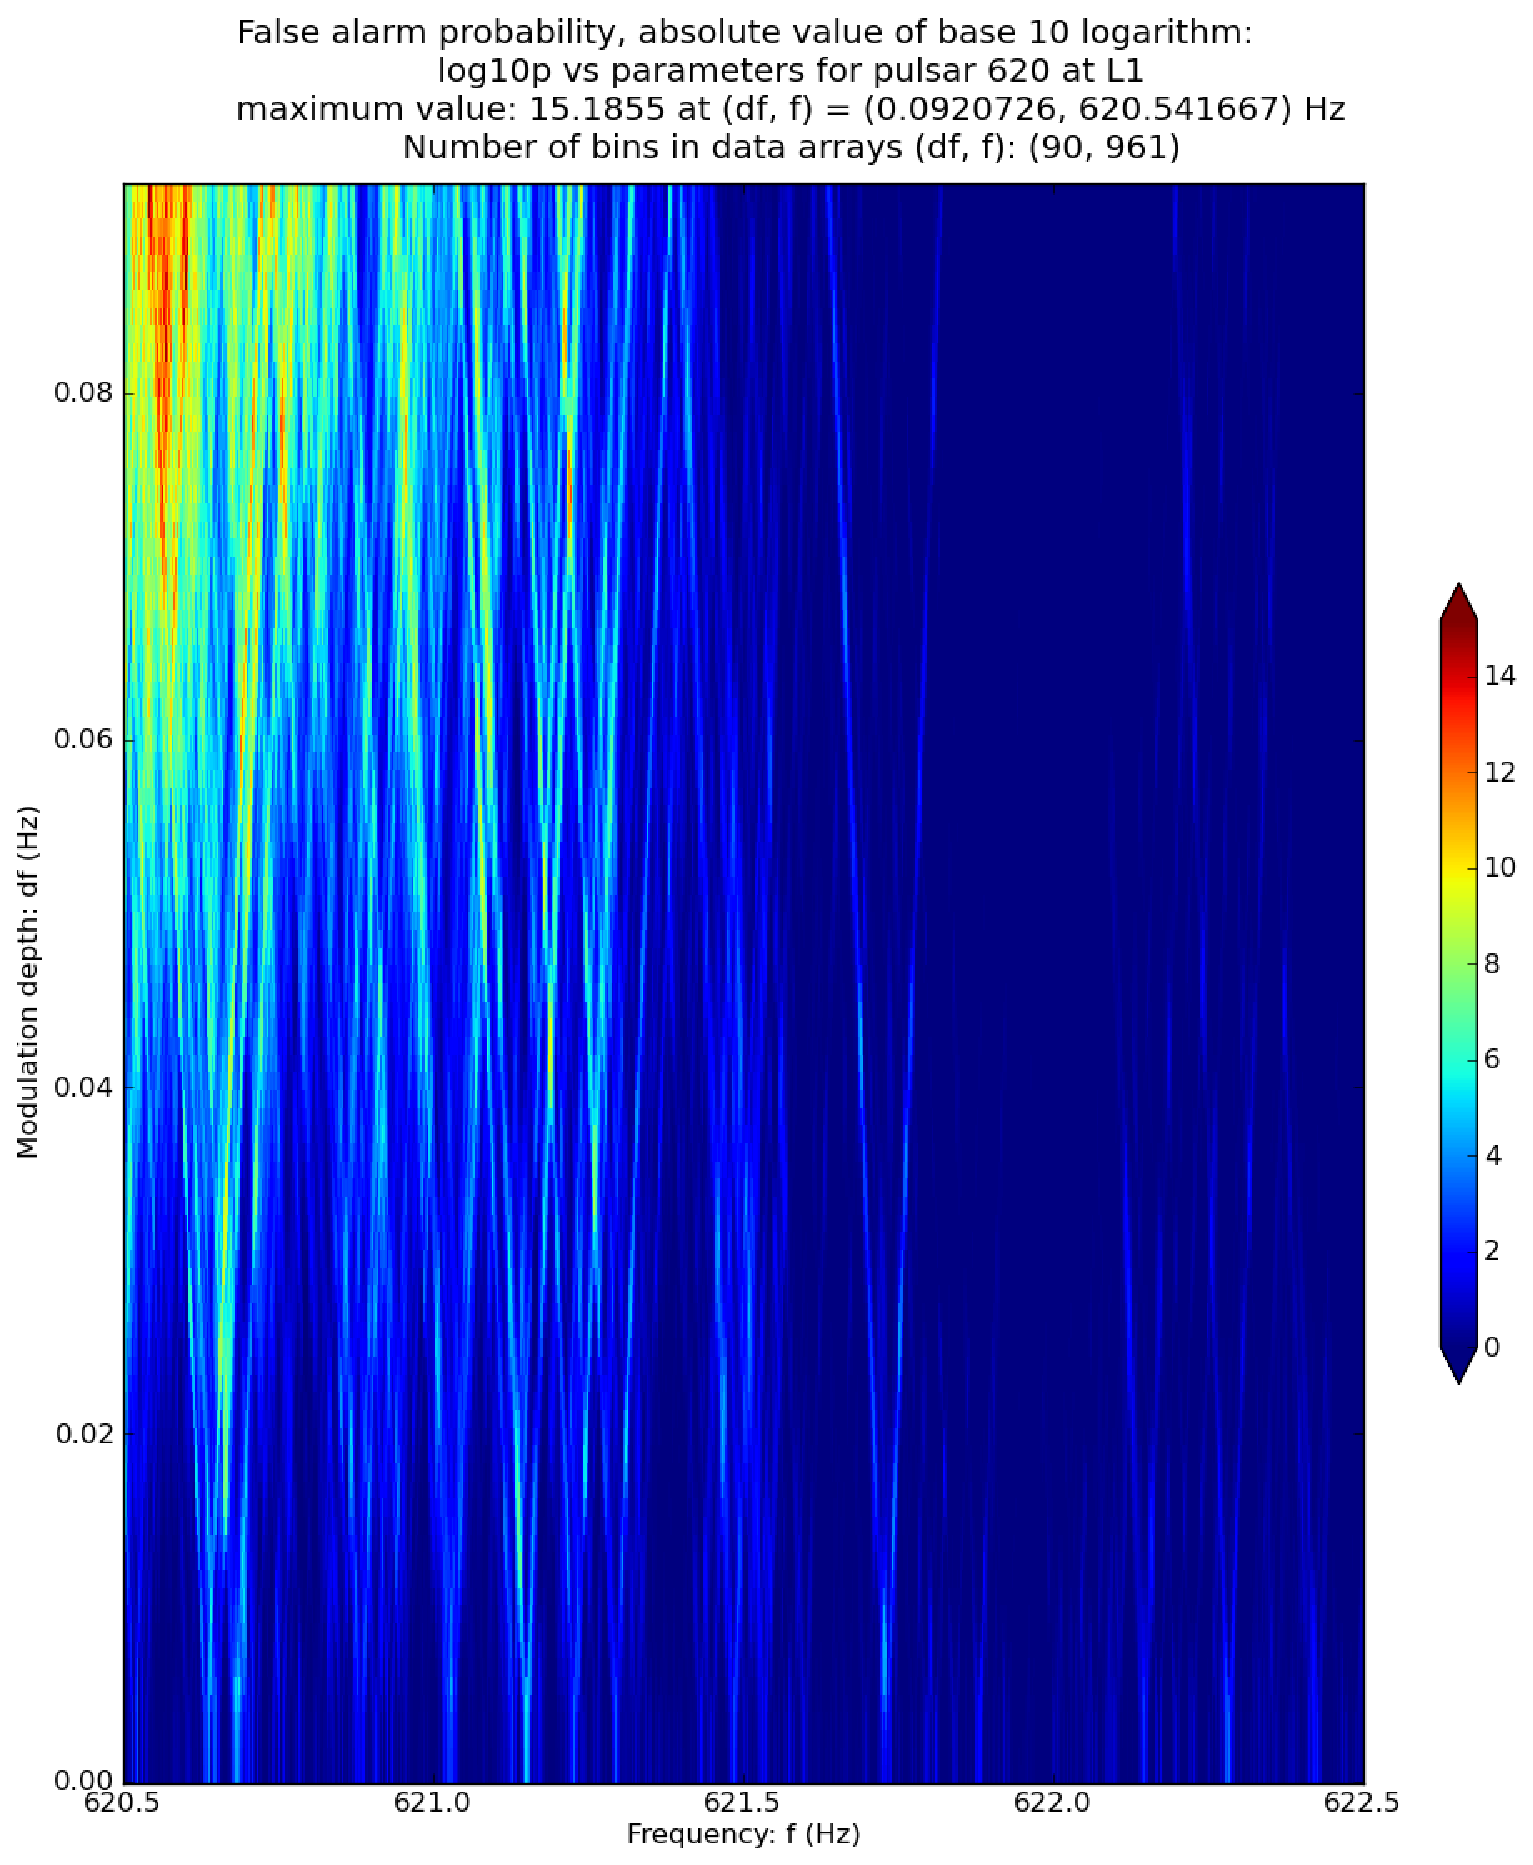
\includegraphics[width=0.4\paperwidth,height=0.2\paperheight]{plots/DFvsFresultsProb-L1_pulsar-620.eps}
\caption{
Quick look at J1751-305, L1 log10p, 621 Hz $r$-mode}
\end{center}
\end{figure}


\section{Summary of Directed TwoSpect S6 searches}

\textbf{2 kHz, $\pm 3 \sigma_{a \sin i}$ search over all S6 data from H1 \& L1}
\begin{itemize}
\item Analyze 40 to 360 Hz with 840 s SFTs,
\item Analyze 360 to 2040 Hz with 360 s SFTs,\\
(to prevent spectral leakage)
\item Now planned: overlapping bands to verify
\item Search over 300+1700 Hz = 2.0 kHz complete on H1
\item Search over 300+1700 Hz = 2.0 kHz complete on L1
\end{itemize}


\emph{S6 search \textbf{100\% done} in 30 days, with 2 kHz per H1, L1}

\begin{enumerate}
\item Should verify overlapping bands with shorter coherence length
\item Refining upper limit methodology
\item R statistic: quiet 0.1 Hz bands need investigation
\item Detection criteria: how applicable is MDC experience?
\end{enumerate}

\emph{Random polarization} $h_0$ lower limit might be $< 1.3\times10^{-24}$
\emph{Outliers} incoming: already $\sim 22$ coincident features in [40, 360] Hz

Plans for O1, first aLIGO run


\textit{As previously noted, results from this chapter are preliminary and have not been reviewed yet by the LIGO Scientific Collaboration.}

        %---------------------------------

	%The following is an example of using the commands \textit{ref}
	%and \textit{label}. With these commands theorems, chapters,
	%sections and figurres can be labeld with names in the tex file
	%and then refered to by these names in later tex files. In
	%chapter~\ref{intro} we saw section~\ref{sample_section} or
	%theorem~\ref{sample_theorem}.

	%Lastly, here is how to include a figure. First generate an
	%encapsulated postscript file in xfig, adobe illustrator or
	%some other program. The specific commands are found in
	%\textit{chap2.tex}.

        %\begin{figure}[htb]
        %\centerline{ \epsfig{figure=sample.eps, 
        %height =  1.5 in}}
        %\caption{Sample Figure}
        %\label{sample_figure}
        %\end{figure}

